\section{Facilidades de Ruby on Rails para cumplir con las reglas de performance}

En esta sección se desarrolla un resumen de cómo \emph{Ruby on Rails} brinda mecanismos y herramientas para poder cumplir con las reglas de performance de forma sencilla y transparente al desarrollador web. Por cada regla relevante se brindará una descripción de lo que ofrece el framework para cumplirla.

\subsection{Realizar menos pedidos HTTP}

Como fue descrito en secciones anteriores, existen varias formas de reducir la cantidad de pedidos necesarios por parte del cliente para cargar un sitio. La mayoría de los
pedidos realizados para lograrlo, son recursos de tipo imagen, hojas de estilo (CSS) y \emph{scripts} (Javascript).

Como ya se detalló en secciones anteriores, uno de los problemas existentes es tener muchos archivos separados de hojas de estilo y \emph{scripts}. Esto genera que el navegador
del usuario deba realizar un pedido por cada uno de los recursos. Sin embargo, tener estos archivos separados favorece la mantenibilidad debido a la modularización, basándose en la
idea de ``divide y vencerás''. De ser necesario unificar todos los archivos en uno, se perderían las características anteriormente mencionadas, tornando el desarrollo más complejo.

Para resolver este problema, a partir de su versión 3.1.0, \emph{Ruby on Rails} brinda un componente llamado \emph{asset pipeline}.  La idea detrás del mismo, es resolver el
problema de unificación de recursos, sin perder las características deseables de practicidad en el desarrollo. Dado el mantra convención sobre configuración, si un desarrollador
sigue las convenciones del \emph{asset pipeline}, obtendrá automáticamente los dos beneficios buscados. Para ello, todos los recursos anteriormente mencionados deberán
estructurarse en la aplicación de la siguiente forma:

\begin{figure}[h]
\centering
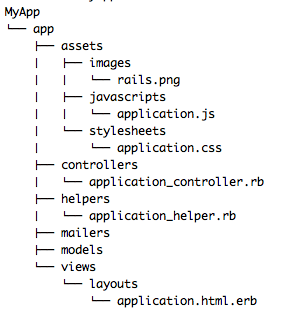
\includegraphics[width=0.5\textwidth]{figuras/rails_app.png}
	\caption{Estructura de aplicación rails típica}
    \label{fig.aplicacion_rails_tipica}
\end{figure}

Dentro del directorio \emph{app/assets} de una aplicación \emph{Rails} típica (ver figura \ref{fig.aplicacion_rails_tipica}), existen por defecto tres directorios:
\emph{images}, \emph{styesheets} y \emph{javascripts}. Como indican sus nombres, el desarrollador deberá introducir los recursos de cada tipo en la carpeta correspondiente. Para
las hojas de estilo y los \emph{scripts} el desarrollador tiene a su disposición una serie de meta funciones que le permiten indicar dependencia entre archivos. Por ejemplo:
Supongamos que el desarrollador tiene dos archivos \emph{javascript}, \emph{principal.js} y \emph{modulo.js}. Para indicar que el archivo \emph{principal.js} requiere al archivo \emph{modulo.js}, dentro
del archivo \emph{principal} debe agregarse una línea con el siguiente contenido, ``//= require modulo''. Esto le indicará al \emph{asset pipeline} cuando realice la compilación de los
recursos, que dentro del archivo \emph{principal.js}, debe incluirse el contenido del archivo \emph{modulo.js}. 

La idea detrás de esto, es que el desarrollador incluya un único archivo de hojas
de estilo y de \emph{scripts} y que en ellos se incluya todo el código de aplicación necesario. Para incluir archivos unificados de recursos, el desarrollador solamente debe
utilizar los métodos que provee \emph{Rails}, \emph{javascript\_include\_tag(script)} y \emph{stylesheet \_link\_tag(hoja de estilo)} en el \emph{layout} más general de la aplicación. El
primer método genera un elemento HTML de tipo \emph{script} con el atributo \emph{src} igual a la ruta del archivo parámetro. El segundo genera un elemento HTML de tipo
\emph{a} con el atributo \emph{href} igual a la ruta de la hoja de estilos unificada.

El \emph{asset pipeline} soluciona este problema para las hojas de estilo y los \emph{scripts}, sin embargo, existe el mismo problema con las imágenes. A priori parecería que seguir
una solución del mismo estilo para las imágenes, no es muy intuitiva. Hay dos tipos de imágenes, las de naturaleza cambiante (por ejemplo, las generadas por usuarios en redes
sociales), y las que se mantienen estáticas en el tiempo, como por ejemplo iconos, logos de empresas, etc. 

Para las imágenes de naturaleza cambiante no hay mucho que hacer, ya
que generalmente no se tiene control sobre ellas. Para las imágenes estáticas existen diferentes técnicas para agruparlas, y que el navegador del usuario deba realizar menos
pedidos. Una de las técnicas ya mencionadas para realizar esta optimización es realizar \emph{CSS sprites}. La idea detrás de esta técnica es unificar las imágenes estáticas en una
única imagen, y que el navegador del usuario realice un único pedido. Luego, por medio de directivas \emph{CSS} desplegar fragmentos de la imagen unificada como si fueran
imágenes individuales.

\emph{Ruby on Rails} no incluye por defecto ningún mecanismo para utilizar esta técnica. Sin embargo, existen paquetes fáciles de incluir en la aplicación que hacen que implementar esta
técnica sea sencillo. Uno de los paquetes disponibles al día de hoy es \emph{compass} \cite{compass}. Para incluir esta dependencia en una aplicación
\emph{Rails}, hay que agregar la siguiente línea en el Gemfile ``gem rails-compass''. Éste paquete genera \emph{CSS sprites} a partir de carpetas de imágenes, realizando el proceso de
unificación de imágenes de manera automática. Además, genera una clase \emph{CSS} por cada imagen perteneciente al \emph{sprite}. Cada clase tiene asignada el atributo
\emph{background-image} a la imagen unificada generada y el atributo \emph{background-position} en el valor adecuado para desplegar la imagen que se encuentra dentro del \emph{sprite}.

Para indicarle a \emph{compass} qué carpeta se desea utilizar para generar el \emph{sprite} se deben agregar las siguientes líneas a la hoja de estilo de la aplicación:
\begin{itemize}

\item @import compass

\item @import 'icons/*.png', esta línea le indica a \emph{compass} que debe unificar en un \emph{sprite} todas las imágenes de tipo PNG dentro de la carpeta icons.

\item @include all-icons-sprites, esta línea le indica a \emph{compass} que debe incluir dentro de la hoja de estilo las clases \emph{CSS} generadas, para que el desarrollador haga uso de
ellas.
\end{itemize}

Por más que \emph{compass} brinde todas estas facilidades, convertir el HTML generado al necesario para utilizar los \emph{sprites} puede tornarse difícil, y puede volver el manejo
de imágenes a futuro un poco más complicado, sin embargo, si se trata de muchas imágenes, la mejora en la reducción de pedidos puede llegar a ser muy significativa.
En futuras secciones se verá la aplicación de \emph{compass} en un caso de estudio de la realidad.

%minificación
\subsection{Minificación}

Otra manera de mejorar la performance en aplicaciones web ligada a los recursos de tipo \emph{javascript} y hojas de estilo, es la minificación de los mismos.
\emph{Rails} otorga esta mejora a través del \emph{asset pipeline} de manera muy transparente, brindando algunas facilidades. Para mantener la comodidad durante el desarrollo,
en los archivos de tipo \emph{script} y hojas de estilo se utilizan espacios, tabulaciones y saltos de línea para mantener la claridad y mantenibilidad en el código. En el ambiente de
desarrollo el \emph{asset pipeline} no realiza minificación alguna, permitiendo que la depuración del código sea más accesible.

 En el ambiente de producción, se realiza la
minificación de estos archivos de manera automática, utilizando por defecto el compresor \emph{uglifier}. El minificador puede cambiarse de manera sencilla, simplemente incluyendo
su paquete en el Gemfile y cambiando la configuración del \emph{asset pipeline} para que lo utilice.

\subsection{Compresión}
\label{cap4:cumpl_rails:compresion}

Con respecto a la regla de compresión, el \emph{asset pipeline} en el ambiente de producción en el momento de compilación además de minificar los recursos, también los comprime
utilizando \emph{gzip}. Luego, es necesario configurar el servidor web para que entregue estos archivos cuando los navegadores realicen pedidos.
Los servidores web son capaces de comprimir los archivos exactamente antes de entregarlos. La facilidad que el \emph{asset pipeline} brinda es la de dejarlos comprimidos,
evitando el trabajo de compresión que de lo contrario hubiera sido necesario realizar por pedido.

\subsection{Expires y Renombrado de archivos}

Una forma de evitar que el navegador realice pedidos innecesarios es explotar al máximo el \emph{cache} del navegador. Para lograr esto, se debe configurar a los servidores web para que
retornen en las respuestas a los pedidos por los recursos el encabezado \emph{Expires}. El objetivo es enviar una fecha de expiración muy adelantada en el tiempo, por ejemplo un
año. Esto se debe a que una vez que el navegador realizó \emph{caching} sobre algún contenido, cada vez que se realice un pedido por dicho recurso, el navegador solo realizará
el pedido si el archivo no ha expirado, ahorrando una enorme cantidad de pedidos innecesarios.
 
El problema que puede surgir es que si el archivo es modificado en el servidor, no hay manera de invalidar el \emph{cache} del navegador, ya que el mismo utiliza
la URL del archivo para guardarlo. Solamente realizará el pedido por ese recurso nuevamente una vez que el mismo haya expirado en su \emph{cache}.
Mediante el \emph{asset pipeline} \emph{Rails} brinda un mecanismo para evitar este problema. 

En el proceso de compilación de los recursos, se calcula una clave md5 basada en el
contenido de cada recurso. A cada recurso se le agrega ésta clave md5 en su nombre de archivo. De esta manera, cuando se produce un cambio en un archivo, la clave md5
generada para el mismo también cambiará, resultando en un cambio en la URL de ese recurso. Este cambio produce que el navegador no sea capaz de detectar que se trata del
mismo archivo. 

Para el desarrollador, toda la complejidad del manejo de las URLs con claves md5 generadas en tiempo de compilación es completamente transparente. Lo
único que debe hacer es utilizar los métodos \emph{javascript\_include\_tag} y \emph{stylesheet\_link\_tag}, con la ruta a los archivos.

\subsection{Utilizar \emph{scripts} y hojas de estilo externas}

Tener el código \emph{javascript} y de hojas de estilo separado del código HTML tiene beneficios, como por ejemplo explotar al máximo el cache del navegador. Sin embargo, tener
muchos archivos externos separados por página, puede traer la desventaja de que el navegador deba realizar un pedido por cada recurso. Como ya se detalló, la convención de
\emph{Rails} lleva a que todos los recursos se unifiquen en un solo archivo por tipo de recurso. Esto explota la ventaja de recursos externos sin sufrir la penalidad de tener muchos
archivos separados.

\subsection{Configurar \emph{Etags}}

Como se indicó en secciones anteriores, el mecanismo de los \emph{Etags} funciona de la siguiente manera. Cuando el navegador realiza un pedido a una página o recurso, en la
respuesta del servidor se incluye un encabezado que identifica al contenido pedido. Este encabezado varía según la implementación del servidor web, por ejemplo en la
implementación de Apache, el \emph{etag} depende del número de i-nodo del recurso en el servidor.

 Uno de los problemas es que si se dispone de varios servidores, el número de inodo de
un mismo recurso varía de servidor a servidor con una probabilidad muy alta. Sin embargo, la implementación de los \emph{Etags} puede ser modificada a nivel de aplicación.
En el caso de los recursos de tipo \emph{script} y hojas de estilo, la convención en \emph{Rails} es deshabilitar los \emph{Etags} para aprovechar los mecanismos de claves md5 
descritos en secciones anteriores. En el caso de otros tipos de recursos como páginas generadas, \emph{Rails} devuelve como \emph{Etag} para dicho recurso, la clave md5 del 
contenido de la respuesta generada. Esta implementación no es susceptible al problema mencionado anteriormente, ya que el contenido del recurso no variará de servidor a servidor.
